\documentclass{standalone}
\usepackage{tikz}
\usepackage{amsmath}
\usetikzlibrary{calc}

\begin{document}

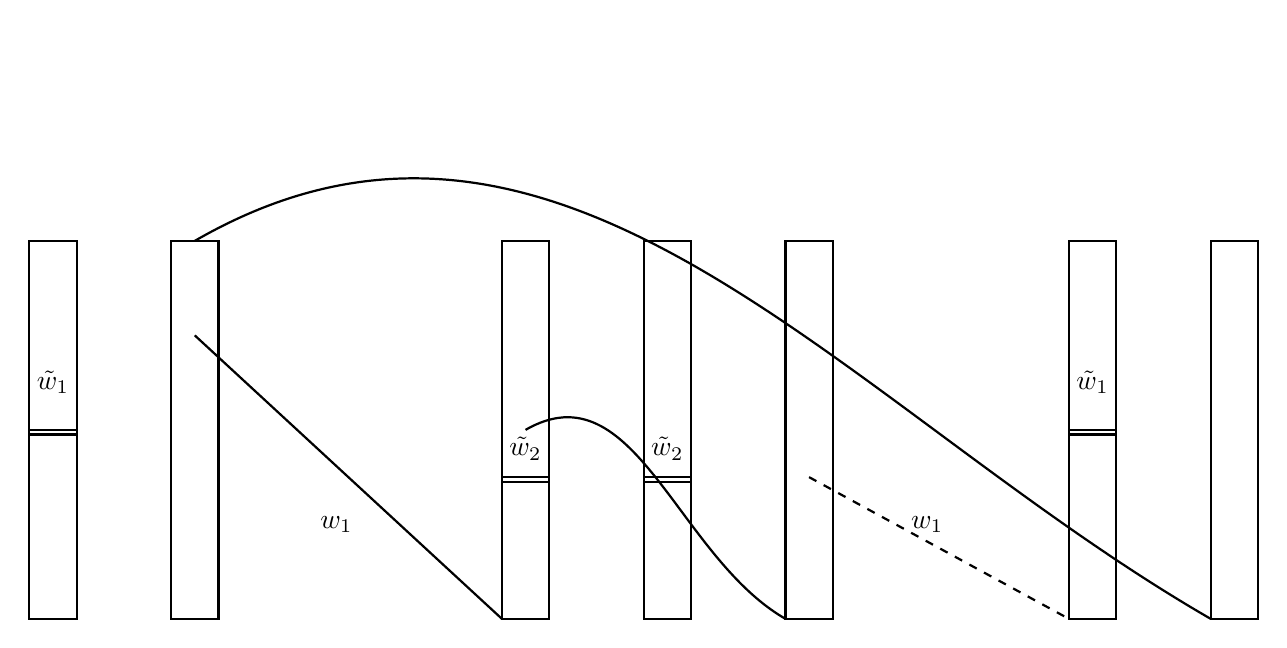
\begin{tikzpicture}[scale=1.2, thick]

% Define coordinates for vertical bars
\coordinate (L1) at (0,0);
\coordinate (L2) at (1.5,0);
\coordinate (M1) at (5,0);
\coordinate (M2) at (6.5,0);
\coordinate (M3) at (8,0);
\coordinate (R1) at (11,0);
\coordinate (R2) at (12.5,0);

% Draw vertical bars
\foreach \x in {L1,L2,M1,M2,M3,R1,R2} {
    \draw (\x) rectangle ++(0.5,4);
}

% Draw horizontal lines within bars
\draw (L1) ++(0,2) -- ++(0.5,0);
\draw (L1) ++(0,1.95) -- ++(0.5,0);
\draw (M1) ++(0,1.5) -- ++(0.5,0);
\draw (M1) ++(0,1.45) -- ++(0.5,0);
\draw (M2) ++(0,1.5) -- ++(0.5,0);
\draw (M2) ++(0,1.45) -- ++(0.5,0);
\draw (R1) ++(0,2) -- ++(0.5,0);
\draw (R1) ++(0,1.95) -- ++(0.5,0);

% Add labels inside bars
\node at ($(L1)+(0.25,2.5)$) {$\tilde{w}_1$};
\node at ($(M1)+(0.25,1.8)$) {$\tilde{w}_2$};
\node at ($(M2)+(0.25,1.8)$) {$\tilde{w}_2$};
\node at ($(R1)+(0.25,2.5)$) {$\tilde{w}_1$};

% Draw top arc connecting left and right groups
\draw (L2) ++(0.25,4) to[out=30, in=150] (R2) ++(-0.25,4);

% Draw middle arc connecting middle bars
\draw (M1) ++(0.25,2) to[out=30, in=150] (M3) ++(-0.25,2);

% Draw diagonal lines
\draw (L2) ++(0.25,3) -- (M1) ++(0.25,1.5);
\draw[dashed] (M3) ++(0.25,1.5) -- (R1) ++(0.25,3);

% Add edge labels
\node at ($(L2)!0.5!(M1)+(0,1)$) {$w_1$};
\node at ($(M3)!0.5!(R1)+(0,1)$) {$w_1$};

\end{tikzpicture}

\end{document}